        \documentclass{standalone}
        \usepackage{tikz}
        \usetikzlibrary{arrows}
        \usepackage{amsmath}
        \usepackage{amsfonts}
        \begin{document}
        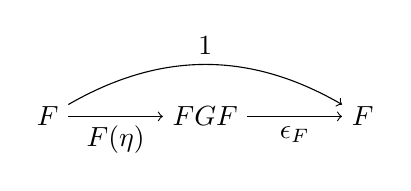
\begin{tikzpicture}

    \node at (0,0) (F1) {$F$};
    \node at (2,0) (FGF) {$FGF$};
    \node at (4,0) (F2) {$F$};
    \draw[->] (F1) -- node[below] {$F(\eta)$} (FGF);
    \draw[->] (FGF) -- node[below] {$\epsilon_F$} (F2);
    \draw[->] (F1) to [out=30,in=150] node[above] {$1$} (F2); 
        \end{tikzpicture}
        \end{document}
